\subsection{Etapa de Prototipação}

O protótipo da interface do usuário será desenvolvida utilizando como base o modelo utilizando no \textit{Montra}, um projeto com design free, ou seja, que pode ser utilizado por qualquer pessoa.

\begin{figure}[!htb]
    \centering
    \caption{Página inicial}
    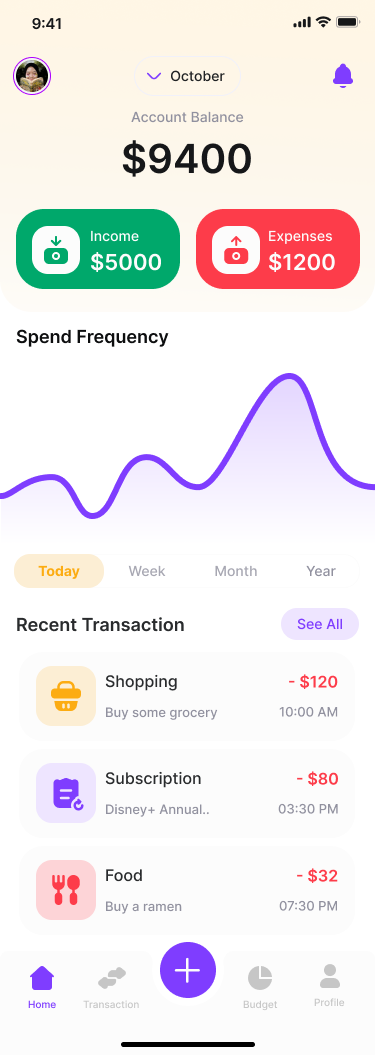
\includegraphics[scale=0.3]{images/Home.png}
\end{figure}

\begin{figure}[!htb]
    \centering
    \caption{Página de adicionar despesa}
    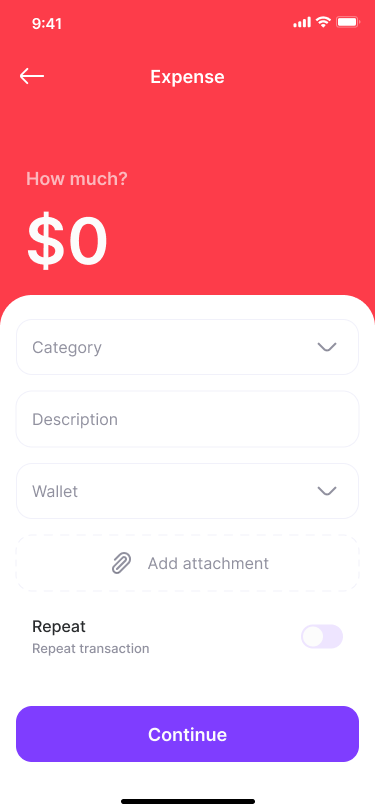
\includegraphics[scale=0.3]{images/expense.png}
\end{figure}

\begin{figure}[!htb]
    \centering
    \caption{Página de adicionar receita}
    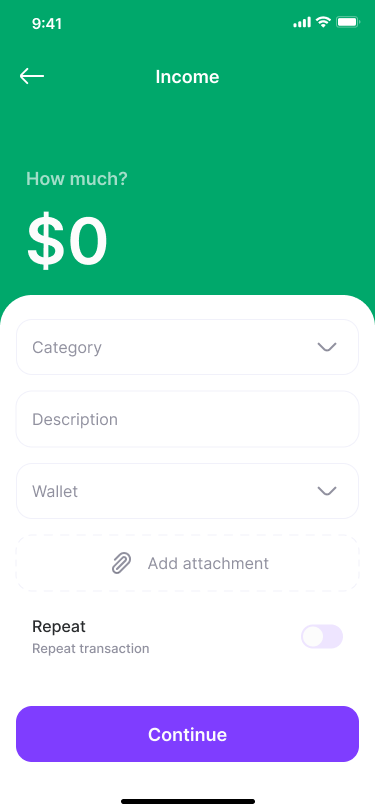
\includegraphics[scale=0.3]{images/income.png}
\end{figure}

\begin{figure}[!htb]
    \centering
    \caption{Página de adicionar notificação}
    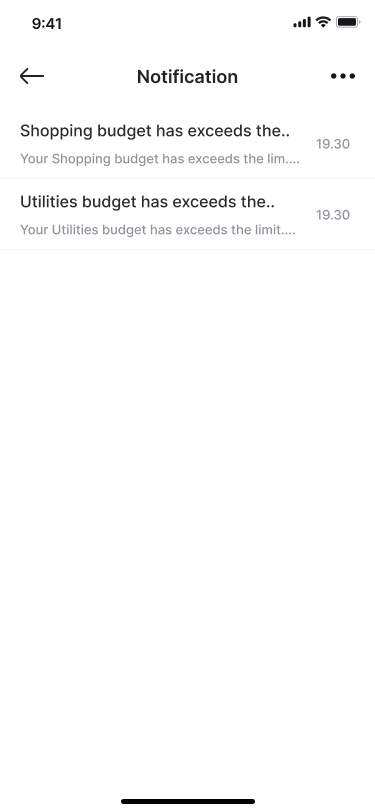
\includegraphics[scale=0.3]{images/Notification.png}
\end{figure}


As figuras mostradas foram apenas uma porção, \textit{sneakpeak} do que foi desenvolvido, o material completo pode ser encontrado no site do figma